%  article.tex (Version 3.3, released 19 January 2008)
%  Article to demonstrate format for SPIE Proceedings
%  Special instructions are included in this file after the
%  symbol %>>>>
%  Numerous commands are commented out, but included to show how
%  to effect various options, e.g., to print page numbers, etc.
%  This LaTeX source file is composed for LaTeX2e.

%  The following commands have been added in the SPIE class 
%  file (spie.cls) and will not be understood in other classes:
%  \supit{}, \authorinfo{}, \skiplinehalf, \keywords{}
%  The bibliography style file is called spiebib.bst, 
%  which replaces the standard style unstr.bst.  

\documentclass[]{spie}  %>>> use for US letter paper
%%\documentclass[a4paper]{spie}  %>>> use this instead for A4 paper
%%\documentclass[nocompress]{spie}  %>>> to avoid compression of citations
%% \addtolength{\voffset}{9mm}   %>>> moves text field down
%% \renewcommand{\baselinestretch}{1.65}   %>>> 1.65 for double spacing, 1.25 for 1.5 spacing 
%  The following command loads a graphics package to include images 
%  in the document. It may be necessary to specify a DVI driver option,
%  e.g., [dvips], but that may be inappropriate for some LaTeX 
%  installations. 
\usepackage[]{graphicx}
\usepackage{amsmath}

\title{Statistical bias in optimized VBM} 

%>>>> The author is responsible for formatting the 
%  author list and their institutions.  Use  \skiplinehalf 
%  to separate author list from addresses and between each address.
%  The correspondence between each author and his/her address
%  can be indicated with a superscript in italics, 
%  which is easily obtained with \supit{}.

\author{Nicholas J. Tustison\supit{a}, Brian B. Avants\supit{b}, Philip A. Cook\supit{b}, James C. Gee\supit{b}, and James R. Stone\supit{a}
\skiplinehalf
\supit{a}Department of Radiology and Medical Imaging, University of Virginia, Charlottesville, Virginia, USA\\
\supit{b}Penn Image Computing and Science Laboratory, University of Pennsylvania, Philadelphia, Pennsylvania, USA
}

%>>>> Further information about the authors, other than their 
%  institution and addresses, should be included as a footnote, 
%  which is facilitated by the \authorinfo{} command.

\authorinfo{Further author information: (Send correspondence to N.J.T.)\\
            N.J.T.: E-mail: njt4n@virginia.edu, Telephone: 1 434 924 7730}
%%>>>> when using amstex, you need to use @@ instead of @
 

%%%%%%%%%%%%%%%%%%%%%%%%%%%%%%%%%%%%%%%%%%%%%%%%%%%%%%%%%%%%% 
%>>>> uncomment following for page numbers
% \pagestyle{plain}    
%>>>> uncomment following to start page numbering at 301 
%\setcounter{page}{301} 
 
  \begin{document} 
  \maketitle 

%%%%%%%%%%%%%%%%%%%%%%%%%%%%%%%%%%%%%%%%%%%%%%%%%%%%%%%%%%%%% 
\begin{abstract}
The recent discovery of methodological flaws in experimental 
design and analysis in neuroscience research has raised concerns 
over the validity of certain 
techniques used in routine analyses and their corresponding 
findings. 
Such concerns have centered around selection bias whereby data is
inadvertently manipulated such that the resulting analysis produces falsely 
increased statistical significance, i.e. type I errors. This has been 
illustrated recently in fMRI studies \cite{vul2009}, with excessive flexibility 
in data collection \cite{simmons2011}, and general experimental design 
issues \cite{kriegeskorte2009}.  Current work from our group has shown
how this problem extends to generic voxel-based analysis (and certain 
technique derivatives such as tract-based spatial statistics\cite{Smith2006}) 
using fractional anisotropy images derived from diffusion tensor imaging \cite{tustison2012}.
In this work, we demonstrate how this circularity principle 
can potentially extend to the well-known
optimized voxel-based morphometry technique \cite{Good2001} for assessing
cortical density differences whereby the principal cause of experimental 
corruption is due to normalization strategy.  Specifically, the popular sum-of-squared-differences (SSD) metric
explicitly optimizes statistical findings potentially inflating type I errors.  
Additional experimentation demonstrates that 
this problem is not restricted to the SSD metric but extends to other commonly
used metrics such as mutual information, neighborhood cross correlation, and
Demons. 
%In the spirit of reproducibility, all experiments were carried out using
%the open source Advanced Normalization Tools (ANTs) software package and 
%a subset of the publicly available IXI dataset.
\end{abstract}

%TThe recent discovery of methodological flaws in experimental design and analysis in neuroscience research has raised concerns over the validity of certain techniques used in routine analyses and their corresponding findings.  Such concerns have centered around selection bias whereby data is inadvertently manipulated such that the resulting analysis produces falsely increased statistical significance, i.e. type I errors. This has been illustrated recently in fMRI studies, with excessive flexibility in data collection, and general experimental design issues.   We demonstrate how this circularity principle  can potentially extend to the well-known optimized voxel-based morphometry technique.

%>>>> Include a list of keywords after the abstract 

\keywords{circularity, cortical thickness, normalization}

%%%%%%%%%%%%%%%%%%%%%%%%%%%%%%%%%%%%%%%%%%%%%%%%%%%%%%%%%%%%%
\section{INTRODUCTION}
\label{sec:intro}  % \label{} allows reference to this section

Voxel-based morphometry (VBM) \cite{wright1995,Ashburner2000} has proven to be
an invaluable technique for the characterization of cortical structural differences 
between populations using neuroimaging data.  Subsequent work
using VBM has explored fundamental neuroscience hypotheses and
has, as a result, become a vital analysis technique in the
neuroscientist's computational toolbox.  
%The core technique of voxelwise comparisons
%in the gray matter between populations has revealed 
%such interesting insights as the relationship between anatomical changes and neuroplasticity 
%\cite{draganski2004},
%the degeneration associated with various neuropathologies \cite{tedeschi2009},
%and other clinically relevant correlations \cite{apkarian2004}.
Briefly, as originally proposed, the standard VBM preprocessing protocol aligns each image to a
T1-weighted template prior to probabilistic segmentation which delineates the white matter, gray matter, 
and cerebrospinal fluid image regions.  Spatial normalization is typically performed on
each subject's T1-weighted image using a global affine normalization procedure to the template
to account for global shape differences followed by deformable registration
to minimize local anatomical differences.  A modification of the standard VBM technique, 
known as ``optimized VBM'', was introduced with the work of Good et al.\cite{Good2001}.  
Instead of spatial normalization to the T1-weighted brain template, an initial 
segmentation occurs in the space of each subject.   The gray matter probability images are then 
normalized to a gray matter
probabilistic template.%
\footnote{
Note that these steps are also applicable to analysis of the white matter.
}  
The normalization parameters are then applied to the corresponding T1-weighted brain 
images.  The remaining portion of the workflow mirrors standard VBM.  

The crucial distinction between the two methods is the normalization step and the images
used to find the transformation between each subject and the template. 
Implicitly quantifying the anatomical differences for many implementations
is the SSD metric.
% which is easily recognized as:
%\begin{align}
%  SSD(\mathcal{I},\mathcal{J},\mathcal{T}) = \frac{1}{N}\sum_{n=1}^N (\mathcal{I}(\mathcal{T}(x_n))-\mathcal{J}(x_n))^2
%\end{align}  
%where $\mathcal{I}$ is the moving image, $\mathcal{J}$ is the fixed image, 
%$\mathcal{T}$ is the transformation to be optimized, and $n$ indexes over the 
%region of interest.  
In fact, the SSD is the metric originally proposed in both methods
and is used in popular, publicly available methods such as SPM2%
\footnote{
http://www.fil.ion.ucl.ac.uk/spm/software/spm2/
}
and FSL-VBM.%
\footnote{
http://www.fmrib.ox.ac.uk/fsl/fslvbm/index.html
}

Closer inspection of the optimization problem of finding the 
set of transformations mapping the entire set of images to the gray
matter template using SSD reveals the circularity of the optimized approach.  
Optimization entails finding the set of $M$ optimal transforms, $\mathcal{T}^*
=\{\mathcal{T}_1, \ldots, \mathcal{T}_M\}$ which maps the $M$ gray 
matter probability images  $\{\mathcal{I}^{gm}_1, \ldots, \mathcal{I}^{gm}_M\}$
to the gray matter template $\mathcal{J}^{gm}$, i.e. 
\begin{align}
  \mathcal{T}^* = \underset{\mathcal{T}_1, \ldots, \mathcal{T}_M}{\operatorname{argmin}}\frac{1}{N}\sum_{m=1}^{M}\sum_{n=1}^N \left(\mathcal{I}^{gm}(\mathcal{T}_m(x_n))-\mathcal{J}^{gm}(x_n)\right)^2.
\end{align}
Switching the summations, 
\begin{align}
  \label{eq:circularity}
  \mathcal{T}^* = \underset{\mathcal{T}_1, \ldots, \mathcal{T}_M}{\operatorname{argmin}}\sum_{n=1}^N 
  \underbrace{\frac{1}{N}\sum_{m=1}^{M}(\mathcal{I}^{gm}\left(\mathcal{T}_m(x_n))-\mathcal{J}^{gm}(x_n)\right)^2}_{\approx average\,\,voxelwise\,\,variance},
\end{align}
 and recognizing that the template gray matter probability
image is a good approximation of the average gray matter probability image, it becomes
apparent that the optimization intended to minimize local shape differences instead, and
more problematically, explicitly minimizes the average variance which directly 
maximizes Student's $t$-test.  Thus, standard preprocessing normalization 
in optimized VBM, instead of maximizing anatomical alignment,  directly manipulates the 
data such that the statistical testing results are maximized which, by 
definition\cite{kriegeskorte2009}, is circular.



%%%%%%%%%%%%%%%%%%%%%%%%%%%%%%%%%%%%%%%%%%%%%%%%%%%%%%%%%%%%%
\section{MATERIALS AND METHODS} 

\begin{figure}
\begin{center}
\begin{tabular}{ccc}
  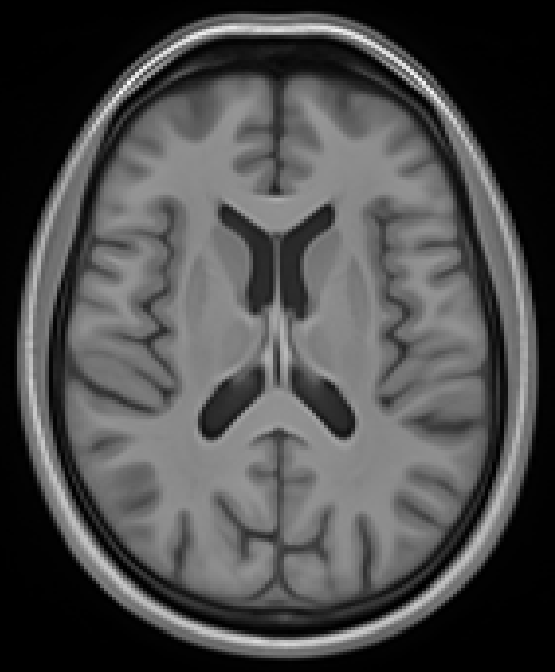
\includegraphics[width=50mm]{atlas.png}&
  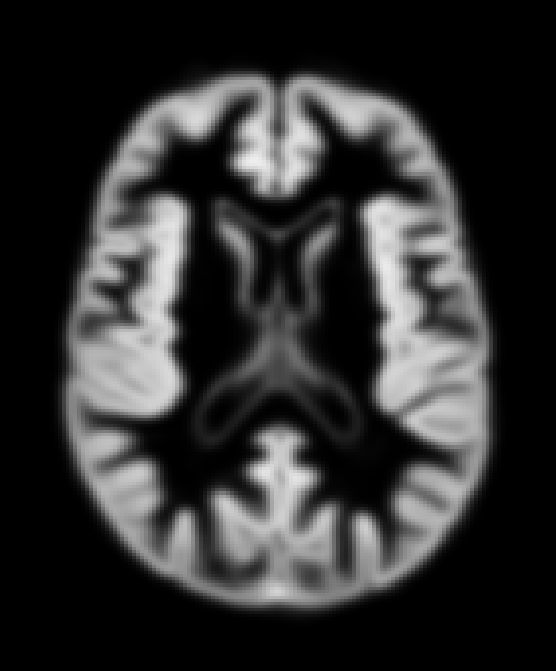
\includegraphics[width=50mm]{atlas_gm.png}&
  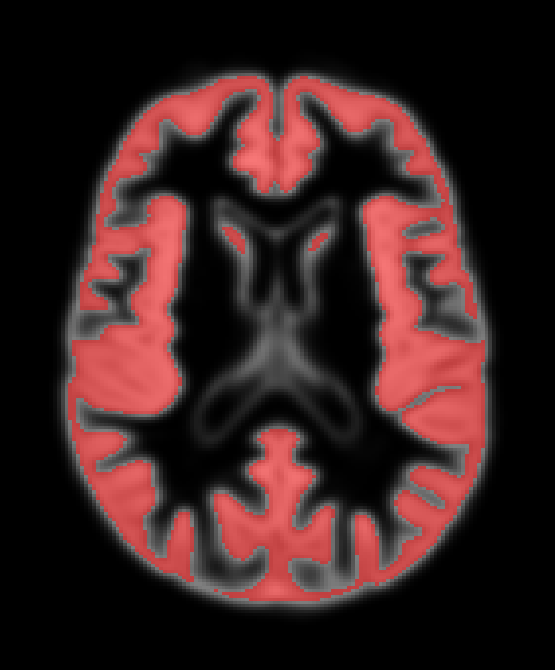
\includegraphics[width=50mm]{atlas_mask.png} \\
  (a) & (b) & (c)
\end{tabular}
\end{center}
\caption{(a) The T1 template created from the set of $56+29=85$ T1 IXI images used in this study.
(b) The gray matter probability template created from the gray matter probability maps.
(c) Mask region defining the domain of the VBM calculations (average gray matter probability $\geq 0.5$).
 }
\label{fig:template}
\end{figure}


Although Eq. (\ref{eq:circularity}) demonstrates the susceptibility 
of the SSD difference metric to producing false positives, we illustrate such 
effects on public data for mutual information (MI), neighborhood cross
correlation (CC), Demons, and SSD.  The relationship of the Demons metric
to SSD would give prior indication that similar effects should 
be seen whereas the effect should be lesser for MI and CC given that the
similarity measures are less localized in addition to not being based on
absolute intensity differences.

\subsection{Images}

Although any of the several high quality public data sets could be used to demonstrate the
presence of circular analysis in optimized VBM, we use the IXI data set consisting
of approximately 600 subjects from three different locations.  Demographic
information including gender and age is also available for each subject.  Further
details can be found on the IXI website.%
\footnote{
http://biomedic.doc.ic.ac.uk/brain-development/
}
For the study in the paper, we used the T1 images from two male subgroups in the age
ranges of 20 to 30 years and 60 to 80 years.  The former subgroup consists of 29 total
images and the latter consists of 56 images.  

\subsection{Generation of Aligned Cohort}

The combined set of T1 images were first used to create an average unbiased shape and 
intensity atlas\cite{Avants2010} (see Fig. \ref{fig:template}(a)). This process also produced a set of transformations
which warps each image to the template space.  Each T1 was then segmented in its native
space using the Atropos\cite{Avants2011a} tool in ANTs. The resulting gray matter
probability maps were then warped to the template space where they were averaged
to create an average gray probability map (denoted as the ``gray matter probability
template'' shown in Fig. \ref{fig:template}(b)).   The two aligned cohorts
were then used to create two sets
of  simulated, aligned gray matter probability maps reflecting the characteristic 
intensities of group. These probability maps were created by calculating the voxelwise
mean and standard deviation of the aligned gray matter probability maps within a
given cohort. The voxel intensity value of the simulated gray matter probability was
then randomly generated using these voxelwise Gaussian parameters.  For our
experiments, we generated 21 synthetic gray matter probability maps from the 20-to-30
group and 20 synthetic gray matter probability maps from the 60-to-80 group.

Using the four similarity metrics described above, we then spatially normalized
each synthetic gray matter probability map to the gray matter probability
template.%
\footnote{
We used the \texttt{antsRegistration} tool also available in ANTs.  Specific common command line
parameters were: \texttt{--convergence [10,0,10] --shrink-factors 1 --smoothing-sigmas 0
--transform SyN[0.5,3,0]}.
}
Despite the fact that each synthetic image was generated in situ 
in the coordinate system of the template, according to the discussion above
in deriving Eq. (\ref{eq:circularity}), optimizing the different similarity metrics will
generate different alignments yielding different VBM results with the SSD and Demons
metric falsely increasing the volume of statistically significant regions.


%%%%%%%%%%%%%%%%%%%%%%%%%%%%%%%%%%%%%%%%%%%%%%%%%%%%%%%%%%%%%
\section{RESULTS} 

Following basic VBM protocol, voxelwise $t$-tests were performed between each
synthetic group over all four metrics and for different levels of smoothing
(0 mm, 4 mm, 8 mm, and 16 mm given in full width at half maximum (FWHM)).  
We then thresholded the resulting $p$-values at $p \leq 0.05$ to yield 
significant regions.  We then calculated the volume of significant regions
for each metric case and compared the volume to the results of
no normalization with the same smoothing level.  The results are shown in 
Table \ref{table:results}.  Positive values are indicative of 
increased statistical significance after spatial normalization.
Whereas the less localized metrics which are not dependent on absolute
intensity differences, i.e. CC and MI, demonstrate a decrease in statistical
significance with normalization, the Demons and SSD metrics 
trend towards a substantial increase in statistically significant volume
as predicted by Eq. (\ref{eq:circularity}).

\begin{table}
\begin{center}
\caption{Change in volume of significant regions relative to 
initial alignment}
\label{table:results}
\begin{tabular*}{0.75\textwidth}{@{\extracolsep{\fill}}ccccc}
{} & 0 mm & 4 mm & 8 mm & 16 mm\\
\hline
MI     & -62\% & -87\% & -91\% & -90\% \\
CC     & -46\% & -58\% & -46\% & -33\% \\
SSD    &  26\% &  14\% & -8\%  &  10\% \\
Demons &  16\% &  27\% & -3\%  &  34\% \\
\hline
\end{tabular*}
\end{center}
\end{table}




%%%%%%%%%%%%%%%%%%%%%%%%%%%%%%%%%%%%%%%%%%%%%%%%%%%%%%%%%%%%%
\section{CONCLUSIONS} 

Spatial normalization is a crucial preprocessing step in many fundamental 
analysis techniques, including optimized VBM.  However, as we point out,
certain normalization strategies (which are commonly used in various 
analyses) are prone to statistical bias by falsely elevating statistical 
significance.  As we have shown, certain metrics such as Demons and SSD,
explicitly optimize the average voxelwise $t$-statistic instead of maximizing
anatomical alignment.  We encourage researchers to reexamine their own
workflow to avoid such problematic practices.

 
%%%%%%%%%%%%%%%%%%%%%%%%%%%%%%%%%%%%%%%%%%%%%%%%%%%%%%%%%%%%%
\section*{APPENDIX} 

Given that the Student's $t$-statistic is estimated from both the group variance
and the difference in group means, an immediate question might concern
the possibility of a concomitant decrease in group mean difference thereby
negating the decrease in group difference caused by group normalization.  
It is important to 
note that it is the {\em average} group variance that goes down 
 and not necessarily the variance at a single voxel site.  Additionally, we can
look at the average group mean difference, $\overline{\Delta\mu}$, over the entire image domain of interest
and manipulate the summation ordering which yields
\begin{align}
  \overline{\Delta\mu}&=\frac{1}{N}\sum_{n=1}^N \left( \mu_1(x_n) - \mu_2(x_n) \right)  \\
  &=\frac{1}{N}\sum_{n=1}^N \left( \frac{1}{M_1}\sum_{m_1=1}^{M_1} \mathcal{I}^{gm}_{m_1}(T_{m_1}(x_n)) - \frac{1}{M_2}\sum_{m_2=1}^{M_2} \mathcal{I}^{gm}_{m_2}(T_{m_2}(x_n)) \right) \\
  &=\left( \frac{1}{M_1}\sum_{m_1=1}^{M_1} \frac{1}{N}\sum_{n=1}^N \mathcal{I}^{gm}_{m_1}\left(T_{m_1}(x_n)\right)\right)
   - \left(\frac{1}{M_2}\sum_{m_2=1}^{M_2} \frac{1}{N}\sum_{n=1}^N \mathcal{I}^{gm}_{m_2}\left(T_{m_2}(x_n)\right)\right).
\end{align}
The inner summations in the two terms make apparent that the average group mean 
difference is dependent solely on how the pixel intensity values are mapped 
within the coordinate space defined by the template. In other words,
$\overline{\Delta\mu}$ depends on the difference between the aggregate intensities
of group 1 and group 2 which is not being directly optimized via minimization of the 
similarity metric (unlike the average group variance). For example, if one combined 
an intensity-preserving transformation 
model with the SSD metric, although the average variance is guaranteed to decrease, the
average group mean difference will remain constant throughout the spatial normalization optimization.


%%%%%%%%%%%%%%%%%%%%%%%%%%%%%%%%%%%%%%%%%%%%%%%%%%%%%%%%%%%%%
%\acknowledgments     %>>>> equivalent to \section*{ACKNOWLEDGMENTS}       
% 
%This unnumbered section is used to identify those who have aided the authors in understanding or accomplishing the work presented and to acknowledge sources of funding.  

%%%%%%%%%%%%%%%%%%%%%%%%%%%%%%%%%%%%%%%%%%%%%%%%%%%%%%%%%%%%%
%%%%% References %%%%%

\bibliography{references}   %>>>> bibliography data in report.bib
\bibliographystyle{spiebib}   %>>>> makes bibtex use spiebib.bst

\end{document} 
